%%%%%%%%%%%%%%%%%%%%%%%%%%%%%%%%%%%%%%%%%%%%%%%%%%%%%%%%%%%%%%%%%%%%
%% I, the copyright holder of this work, release this work into the
%% public domain. This applies worldwide. In some countries this may
%% not be legally possible; if so: I grant anyone the right to use
%% this work for any purpose, without any conditions, unless such
%% conditions are required by law.
%%%%%%%%%%%%%%%%%%%%%%%%%%%%%%%%%%%%%%%%%%%%%%%%%%%%%%%%%%%%%%%%%%%%

\documentclass[
  digital, %% This option enables the default options for the
           %% digital version of a document. Replace with `printed`
           %% to enable the default options for the printed version
           %% of a document.
  twoside, %% This option enables double-sided typesetting. Use at
           %% least 120 g/m² paper to prevent show-through. Replace
           %% with `oneside` to use one-sided typesetting; use only
           %% if you don’t have access to a double-sided printer,
           %% or if one-sided typesetting is a formal requirement
           %% at your faculty.
  table,   %% This option causes the coloring of tables. Replace
           %% with `notable` to restore plain LaTeX tables.
  lof,     %% This option prints the List of Figures. Replace with
           %% `nolof` to hide the List of Figures.
  lot,     %% This option prints the List of Tables. Replace with
           %% `nolot` to hide the List of Tables.
  %% More options are listed in the user guide at
  %% <http://mirrors.ctan.org/macros/latex/contrib/fithesis/guide/mu/fi.pdf>.
]{fithesis3}
%% The following section sets up the locales used in the thesis.
\usepackage[resetfonts]{cmap} %% We need to load the T2A font encoding
\usepackage[T1,T2A]{fontenc}  %% to use the Cyrillic fonts with Russian texts.
\usepackage{epsfig}

\usepackage[
  main=czech, %% By using `czech` or `slovak` as the main locale
                %% instead of `english`, you can typeset the thesis
                %% in either Czech or Slovak, respectively.
  english, german, russian, slovak %% The additional keys allow
]{babel}        %% foreign texts to be typeset as follows:
%%
%%   \begin{otherlanguage}{german}  ... \end{otherlanguage}
%%   \begin{otherlanguage}{russian} ... \end{otherlanguage}
%%   \begin{otherlanguage}{czech}   ... \end{otherlanguage}
%%   \begin{otherlanguage}{slovak}  ... \end{otherlanguage}
%%
%% For non-Latin scripts, it may be necessary to load additional
%% fonts:
\usepackage{paratype}
\def\textrussian#1{{\usefont{T2A}{PTSerif-TLF}{m}{rm}#1}}
%%
%% The following section sets up the metadata of the thesis.
\thesissetup{
    date          = \the\year/\the\month/\the\day,
    university    = mu,
    faculty       = fi,
    type          = bc,
    author        = {Jan Laštůvka},
    gender        = m,
    advisor       = {RNDr. Jan Vykopal, Ph.D.},
    title         = {Aplikace pro hodnocení kyberbezpečnostního cvičení},
    %%TeXtitle      = {The Proof of $\mathsf{P}=\mathsf{NP}$},
    keywords      = {application, CSIRT-MU, implementation, innovation, KYPO, security, SOBHA, visualization},
    TeXkeywords   = {application, CSIRT-MU, implementation, innovation, KYPO, security, SOBHA, visualization},
    abstract      = {V rámci této bakalářské práce byla navržena a implementována nová aplikace pro hodnocení akcí účastníků kyberbezpečnostního cvičení, která nahradí stávající aplikaci používanou v prostředí KYPO. V teoretické části práce je nejdříve představeno cvičení Cyber Czech, kde se tento software používá a následně je proveden rozbor dříve vytvořené aplikace. Na základě zjištěných nedostatků a nově definovaných požadavků je navržen datový model a k tomuto datovému modelu je poté vytvořen návrh aplikačního programového rozhraní. V rámci praktické části je navržená aplikace implementována za pomocí Django REST Framework. V závěru práce je provedeno zhodnocení z reálného použití aplikace a nakonec jsou stanoveny další doporučení pro rozvoj aplikace.},
    thanks        = {These are the acknowledgements for my thesis, which can

                     span multiple paragraphs.},
    bib           = {references-mendeley.bib, bibliography.bib}, 
}
\usepackage{makeidx}      %% The `makeidx` package contains
\makeindex                %% helper commands for index typesetting.
%% These additional packages are used within the document:
\usepackage{paralist} %% Compact list environments
\usepackage{amsmath}  %% Mathematics
\usepackage{amsthm}
\usepackage{amsfonts}
\usepackage{url}      %% Hyperlinks
\usepackage{markdown} %% Lightweight markup
\usepackage{listings} %% Source code highlighting
\lstset{
  basicstyle      = \ttfamily,%
  identifierstyle = \color{black},%
  keywordstyle    = \color{blue},%
  keywordstyle    = {[2]\color{cyan}},%
  keywordstyle    = {[3]\color{olive}},%
  stringstyle     = \color{teal},%
  commentstyle    = \itshape\color{magenta}}
\usepackage{floatrow} %% Putting captions above tables
\floatsetup[table]{capposition=top}

\begin{document}

\chapter*{Úvod}
\addcontentsline{toc}{chapter}{Úvod}

Kybernetické útoky, snažící se prolomit zabezpečení počítačových systémů, narůstají na intenzitě a komplexnosti. Z tohoto důvodu rostou i nároky kladené na správce těchto systémů. Ti musí být schopni systémy vhodně zabezpečit a dokázat reagovat na jakoukoliv formu kybernetického útoku. Jejich znalosti a zkušenosti jsou rozhodujícím faktorem při prevenci proti útokům, ale také při řešení situací spojených s probíhajícím útokem.

Vhodnou metodou vzdělávání jsou kybernetická bezpečnostní cvičení, při kterých účastníci soutěží s ostatními týmy. Vyzkouší si nejen své znalosti a schopnosti rychle reagovat na hrozící útoky, ale také si například osvojí vedení komunikace s médii nebo orgány činnými v trestním řízení.

Jedním z těchto cvičení je i Cyber Czech, které je prozatím jediné pravidelně pořádané cvičení svého druhu v České republice. \cite{cyberex} Akce probíhá v Kybernetickém polygonu Masarykovy univerzity, který vznikl v roce 2015. Tento prostor nabízí technické prostředky pro vytvoření plně funkčních počítačových sítí a zařízení, která se v nich nachází ve virtuálním prostředí.

Předmětem této práce je na míru vytvořený software, který je na cvičeních Cyber Czech používán k hodnocení účastníků a umožňuje vyhodnocovat výsledky z tohoto cvičení. Původní program vykazoval nedostatky, které jsou v práci podrobně rozebrány, a na jejich základě s uvážením nových požadavků je navržena a implementována nová aplikace. Aplikace byla rozdělena na dva samostatné celky. Servisní vrstvu, jejíž návrh a vývoj je předmětem této práce, a prezentační vrstvu vytvořenou v rámci jiné práce. Oba tyto celky spolu komunikují díky aplikačnímu programovému rozhraní servisní vrstvy. 

\chapter{Kyberbezpečnostní cvičení Cyber Czech}

Žijeme v digitalizované době, kdy se internet stal součástí života více než jedné poloviny populace \cite{worldStats}. Pomocí internetu můžeme přistupovat nejen k jednoduchým webovým stránkám, ale také k mnohem komplexnějším informačním systémům. Všechny tyto systémy, komunikující pomocí internetu, jsou však v ohrožení útočníků, kteří se je mohou pokusit kompromitovat nebo do nich proniknout. Kybernetické útoky jsou stále intenzivnější a mnohem komplexnější a je tedy potřeba stále více kyberbezpečnostních profesionálů. Pro tyto profesionály jsou nezbytné nejen znalosti nejrůznějších typů útoků a způsoby, jak se proti těmto útokům bránit. Neméně důležité jsou také zkušenosti s obranou proti reálným útokům, kdy tito odborníci musejí ve stresové situaci a v co nejkratším čase odvrátit probíhající útok nebo alespoň minimalizovat možné dopady. Z tohoto důvodu se stávají stále populárnější kyberbezpečnostní cvičení, kde účastníci mohou znalosti a zkušenosti získávat pomocí aktivního zapojení do cvičení.

\section{Kybernetický polygon Masarykovy univerzity}

Kybernetický polygon Masarykovy univerzity (zkráceně KYPO) vznikl jako projekt s unikátním prostředím uzpůsobeným pro výzkum, vývoj a analýzu hrozeb v oboru informační bezpečnosti a bezpečnosti kritických informačních infrastruktur. Provádí se v něm školení a cvičení počítačové bezpečnosti, výzkum ochrany proti kybernetickým útokům, forenzní analýzy a bezpečnostní experimenty nad počítačovými sítěmi.

KYPO je navržen jako modulární distribuovaný systém. \cite{Vykopal2017KYPOCases} Virtuální prostředí KYPO je vytvořeno v cloudu, díky tomu je možné velice rychle a opakovaně vytvářet nové funkční počítačové sítě a zařízení v těchto sítích. Stejně tak je možné velice snadno provádět údržbu těchto sítí a zařízení. Díky uzavřenému virtuálnímu prostředí KYPO je možné, aby uživatelé mohli ve vytvořených sítích bezpečně provádět jakékoliv experimenty, aniž by mohly být ovlivněny počítačové systémy mimo toto prostředí.


\subsection{Využití kybernetického polygonu}
Díky technologiím, které jsou v KYPO dostupné, nachází tento systém všestranné využití. 
\begin{itemize}
\item Výzkum a vývoj -- v KYPO probíhá výzkum, vývoj a testování nových metod a systémů pro detekci a zmírnění počítačových útoků v různých síťových infrastrukturách.
\item Forenzní analýzy -- díky plně virtuálnímu prostředí a nástrojům, které umožňují monitorování napříč celým vytvořeným systémem, je možné provádět základní forenzní analýzy. Uživatelé mohou spustit virtuální obraz neznámého nebo napadeného stroje v předdefinovaném prostředí a díky nástrojům, které jsou ve virtuálním prostředí dostupné, mohou provádět analýzy takového stroje. 
\item Výuka a kyberbezpečnostní cvičení -- dále KYPO slouží pro výuku v rámci studia na Masarykově univerzitě a také zde probíhá kyberbezpečnostní cvičení Cyber Czech.
\end{itemize}

\section{Kyberbezpečnostní cvičení Cyber Czech}
Cyber Czech je kyberbezpečnostní cvičení, pořádané Ústavem výpočetní techniky Masarykovy univerzity spolu s Národním centrem kybernetické bezpečnosti, který je součástí Národního bezpečnostního úřadu. Jedná se o cvičení, které je postaveno na principu, kdy proti sobě stojí dva týmy, tým modrý (bránící) a tým červený (útočící). Cílem červeného týmu je napadnout různé systémy ve virtuální infrastruktuře modrého týmu, který se naopak snaží proti těmto útokům ubránit. Během cvičení jsou ověřovány technické znalosti členů modrého týmu, ale zároveň jsou zkoušeny i jejich schopnosti jednání ve stresových situacích a v časové tísni. Kromě technických dovedností musejí členové modrých týmů například zvládat komunikovat s fiktivními novináři, policií nebo legitimními uživateli jejich systému.

Jedná se o cvičení, zahrnující aktivní formu účasti, které je určeno odborníkům z řad správců počítačových systémů. Cvičení je postaveno především na principu obrany před útočníky, kteří vykonávají útoky podle předem připraveného scénáře. Útočníci jsou plně seznámeni se síťovou infrastrukturou modrého týmu a veškerá slabá místa, která útočící tým zneužívá, jsou pečlivě předem připravena. Celé cvičení je řízeno fiktivním scénářem, který je všem účastníkům předem představen. Mimo samotný příběh cvičení, jsou účastníci předem seznámeni se síťovou infrastrukturou, kterou musí zabezpečovat, a před samotným zahájením cvičení mají také účastníci prostor k tomu, aby provedli iniciální zabezpečení svěřené sítě.

Cvičení se typicky účastní šest modrých týmů a každý z těchto týmů spravuje zcela identickou počítačovou síť. Červený tým poté na síť každého modrého týmu provádí stejné typy útoků. Celé cvičení pak probíhá formou soutěže mezi těmito šesti týmy, kdy týmy začínají s jistým bodovým základem a během cvičení mohou různými způsoby získávat, nebo naopak ztrácet body. Vítězným týmem je ten, který má na konci cvičení nejvíce bodů. Soutěžní mód cvičení může ovlivňovat hladinu stresu účastníků a vyvíjet tak napětí a stres, které jsou přítomny při zvládání reálných situací.

Ke správě skóre modrých týmů během cvičení slouží skórovací aplikace, jejíž inovace je předmětem této bakalářské práce. 

\subsection{Účastníci cvičení}
Účastníci cvičení jsou rozděleni do čtyř skupin podle jejich úlohy při cvičení.

\begin{itemize}
\item Modrý tým -- tým lidí, kteří jsou v průběhu cvičení zkoušeni. Během cvičení se musí řídit pravidly cvičení a také zákony vztahujícími se na kybernetickou bezpečnost, tedy například ohlašovací povinností kybernetických bezpečnostních incidentů.
\item Červený tým -- tým útočníků, složený z odborníků na kybernetickou bezpečnost. 
\item Bílý tým -- tým lidí, kteří se starají o organizaci a průběh cvičení. Dohlížejí na dodržování pravidel cvičení, na vývoj situace mezi červeným týmem a modrými týmy a dále zajišťují podporu pro modré týmy, pokud mají nějaké dotazy. Simulují média, která podle probíhajícího scénáře cvičení vznáší na modré týmy dotazy. Dále simulují právní poradce, orgány činné v trestním řízení a jiné fiktivní instituce vystupující ve scénáři.
\item Blondýny -- tým lidí, kteří představují reálné uživatele systémů, o které se modré týmy starají. Provádějí legitimní operace a modrý tým musí zajistit, aby systémy, se kterými pracují, byly vždy dostupné.
\item Zelený tým -- tým lidí, spravující celou infrastrukturu používanou na cvičení. Jsou zodpovědní za konfiguraci všech virtuálních počítačů a sítí, za monitoring sítí a za skórovací infrastrukturu. Na žádost modrého týmu mohou provést servisní zásah v jejich síti, typicky obnovení požadovaného stroje do stavu před zahájením cvičení.
\end{itemize}

\subsection{Skórovací aplikace}
Pro hodnocení účastníků cvičení Cyber Czech slouží na míru vytvořený software, který je dostupný jako webová stránka a umožňuje zadávání hodnocení pro modré týmy a nabízí přehledné zobrazení aktuálního skóre všech modrých týmů. Do programu mají přístup všichni účastníci cvičení, kteří zadávají hodnocení modrým týmům. Z toho vyplývá, že modré týmy do aplikace přístup nemají. Modrým týmům je během cvičení promítáno celkové skóre, ve kterém se mohou dozvědět základní informace o svém bodovém zisku a mohou zjistit své pořadí vzhledem k ostatním týmům. Komplexnější zpětná vazba je účastníkům poskytována až po skončení cvičení \cite{Vykopal2017TimelyExercises}.

\subsection{Hodnocené oblasti}
Během cvičení získávají modré týmy hodnocení, na kterém závisí jejich umístění ve výsledném pořadí. Hodnocení je rozděleno do několika složek.

\begin{itemize}
\item Hodnocení pomocí automatického skórování -- během cvičení je pomocí automatických systémů kontrolováno, zda v systému, který modrý tým spravuje, jsou dostupné všechny legitimní služby. Jedná se například o e-mailové servery, webové služby a jiné prvky spravovaných systémů. Modré týmy jsou poté bodově penalizovány za případnou nedostupnost těchto služeb.
\item Hodnocení od červeného týmu -- během cvičení provádí červený tým útoky podle předem naplánovaného scénáře. Do skórovací aplikace poté červený tým zadává bodovou penalizaci za útoky, které se zdařily.
\item Hodnocení od bílého týmu -- bílý tým představuje fiktivní média, orgány činné v trestním řízení, ale zastupuje také roli koordinátora cvičení. Hodnotí převážně intenzitu a formu komunikace. Bílý tým může zadávat záporné hodnocení za nedostatečnou komunikaci, nebo naopak kladné hodnocení za vhodnou komunikaci.
\item Hodnocení od blondýn -- při cvičení je nezbytné, aby systémy byly neustále dostupné legitimním uživatelům. V případě, že systémy nejsou dostupné, případně neumožňují uživatelům plnohodnotné použití, zadávají blondýny modrému týmu bodovou penalizaci.
\item Hodnocení od zeleného týmu -- v případě, že modrý tým narazí na problémy, které není schopen vyřešit, má možnost si vyžádat servisní zásah od organizátorů cvičení, za každou opravu v infrastruktuře modrého týmu zelený tým odečte body danému týmu.
\end{itemize}

\subsection{Základní síťová infrastruktura cvičení}
Jak lze vidět na obrázku \ref{fig:kypoNetwork}, síť vytvořená pro potřeby cvičení je rozdělena do dvou podsítí, kterým se budu věnovat v následujících bodech.

\begin{itemize}
    \item Globální síť -- představuje společnou síťovou infrastrukturu, ve které se nachází např. DNS nebo e-mailové servery. Jedná se o simulaci veřejného internetu, ve kterém se nachází jak útočníci, tak legitimní uživatelé systému. V síti se nachází skórovací aplikace, kterou se budu později blíže zabývat. Aby mohli účastníci cvičení například stahovat bezpečnostní aktualizace nebo vyhledávat potřebné informace na webových serverech, je tato síť připojena také k veřejnému internetu.
    \item Sítě modrých týmů -- každý modrý tým má k dispozici identickou síť, která je pomocí brány připojena do globální sítě. Každá síť modrého týmu obsahuje kritickou infrastrukturu a zranitelné služby, které se snaží napadnout červený tým. Síť modrých týmů je dále rozdělena do několika celků na demilitarizovanou zónu (DMZ), pracovní stanice a servery. V síti je přítomna monitorovací služba, která sleduje síťový provoz, a do této služby je integrována logovací infrastruktura. Každý stroj v síti je poté nakonfigurován tak, aby zapisoval do centrálního logovacího serveru veškeré změny stavu této služby \cite{CeledaKYPO-AExercises}. Monitorovací infrastruktury využívá skórovací aplikace, která na základě zjištěných nedostupností určitých služeb v síti modrého týmu vytváří bodové penalizace pro tento tým.
\end{itemize}

\begin{figure}[h]
    \centering
    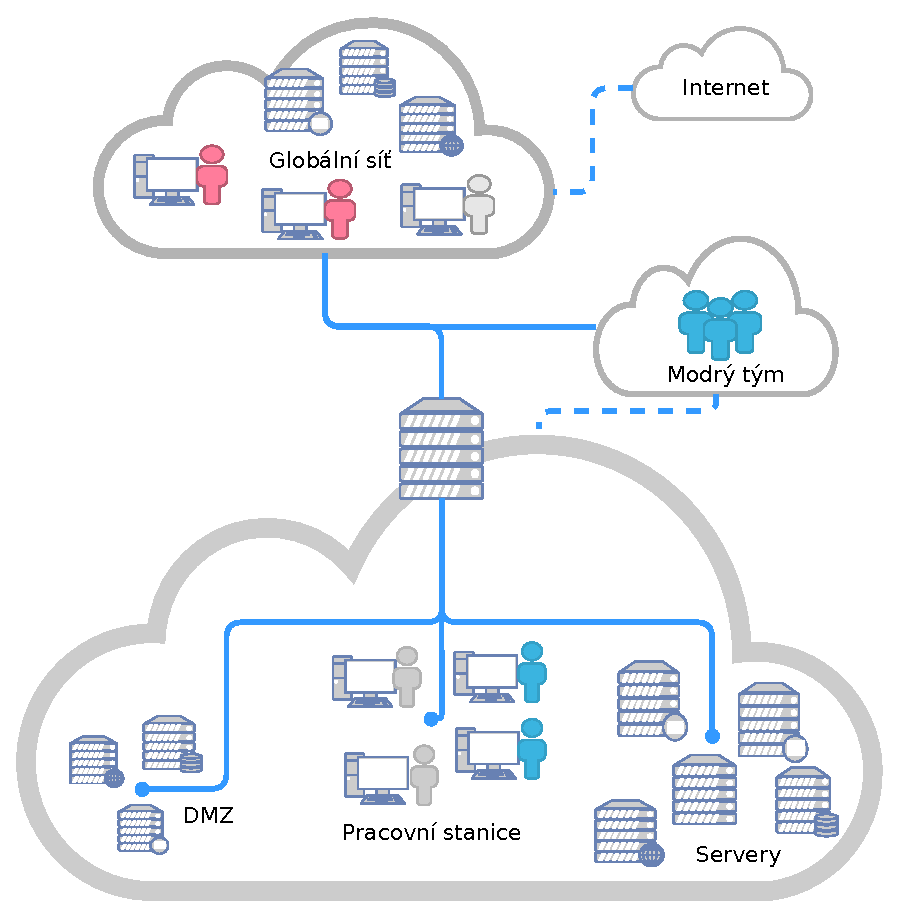
\includegraphics[width=10cm]{images/kypo-network.eps}
    \caption{Schéma znázorňující rozvržení sítě při kybernetickém cvičení Cyber Czech \cite{Vykopal2017LessonsRange}}
    \label{fig:kypoNetwork}
\end{figure}


\chapter{Rozbor původní aplikace}
\section{Návrh aplikace}

Původní aplikace pro hodnocení účastníků kyberbezpečnostního cvičení Cyber Czech byla navržena v rámci diplomové práce Bezpečnostní cvičení v prostředí KYPO, kterou zpracoval Mgr. Milan Kostelník \cite{Kostelnik2016thesis}. V rámci zmíněné diplomové práce byl navržen model hodnocení účastníků cvičení, byly stanoveny funkční požadavky na skórovací aplikaci a dále byl navržen datový model a základní požadavky na grafické zpracování aplikace. Implementace navržené aplikace byla zajištěna Ústavem výpočetní techniky Masarykovy univerzity. Výsledná implementace aplikace se však v nejrůznějších detailech lišila od původního návrhu. V rozboru proto dále analyzuji reálně vytvořenou aplikaci.  

\section{Použité technologie}
Pro implementaci skórovací aplikace byl zvolen programovací jazyk Python s použitím frameworku Django, který je určen pro tvorbu webových systémů. Nyní blíže popíšu tyto technologie a důvody pro jejich použití.

\subsection{Python}
Python je dynamicky interpretovaný programovací jazyk. Vývoj aplikací v Pythonu je rychlý a jeho použití je možné na většině běžných platforem (Unix, Microsoft Windows, macOS). Python lze využít jak pro psaní krátkých skriptů, tak pro vybudování komplexních systémů. Toho bylo v softwaru využito pro naprogramování skriptu pro obsluhu automatického skórování a zároveň vybudování komplexní skórovací aplikace. Pro Python existuje velké množství již hotových knihovních modulů, usnadňujících vývojáři rutinní úlohy. Jedním z těchto modulů je i framework Django, pomocí kterého je skórovací software vytvořen.

\subsection{Django}

Django je open source webový framework, jehož hlavní úlohou je zjednodušit a urychlit vývoj komplexních webových aplikací napojených na databázový systém. Tento systém byl zvolen pro svoji jednoduchost a nabízené výhody, které nyní shrnu. Framework umožňuje snadné budování Model-view-controller (MVC) softwarové architektury a vytvářet tak přehledně strukturovaný kód. Obsahuje propracovaný systém pro objektově relační mapování (ORM), které zajišťuje konverzi dat mezi relační databází a objektově orientovanou aplikací. Při vývoji je tak programátorovi ulehčena práce s databázovou vrstvou. Další výhodou je možnost generování automatické administrace pro datový model vytvořený pomocí Django ORM. Framework obsahuje propracovaný systém pro autentizaci a autorizaci uživatelů. 

\section{Požadavky na skórovací aplikaci}

\subsection{Systémové požadavky}
Pro zajištění co nejjednodušší přístupnosti aplikace bylo požadováno, aby systém měl webové rozhraní, do kterého se mohou účastníci cvičení přihlašovat a zadávat manuální hodnocení.

\subsection{Funkční požadavky}
Na aplikaci bylo stanoveno několik funkčních požadavků \cite{Kostelnik2016thesis}.
\begin{itemize}
\item Kontrola dostupnosti legitimních služeb musí probíhat automaticky a v reálném čase.
\item Aplikace bude umožňovat zadání manuálního hodnocení k událostem, které jsou prováděny červeným týmem, bílým týmem, legitimními uživateli nebo organizátory cvičení.
\item Pro každou událost je nezbytné, aby bylo možné specifikovat dolní a horní mez bodového ohodnocení.
\item Po odeslání hodnocení bude možné provést jeho opravu, případně zpětné odstranění.
\item Systém umožní provádět správu uživatelů pomocí uživatelských rolí. Uživateli pak bude umožněno odeslat hodnocení pouze za události, které může daný tým hodnotit.
\item Systém umožní zobrazení časomíry pro odpočet času do ukončení cvičení.
\end{itemize}

Funkční požadavky shrnuje diagram případů užití na obr. \ref{fig:useCase1}.

\begin{figure}[h!]
    \centering
    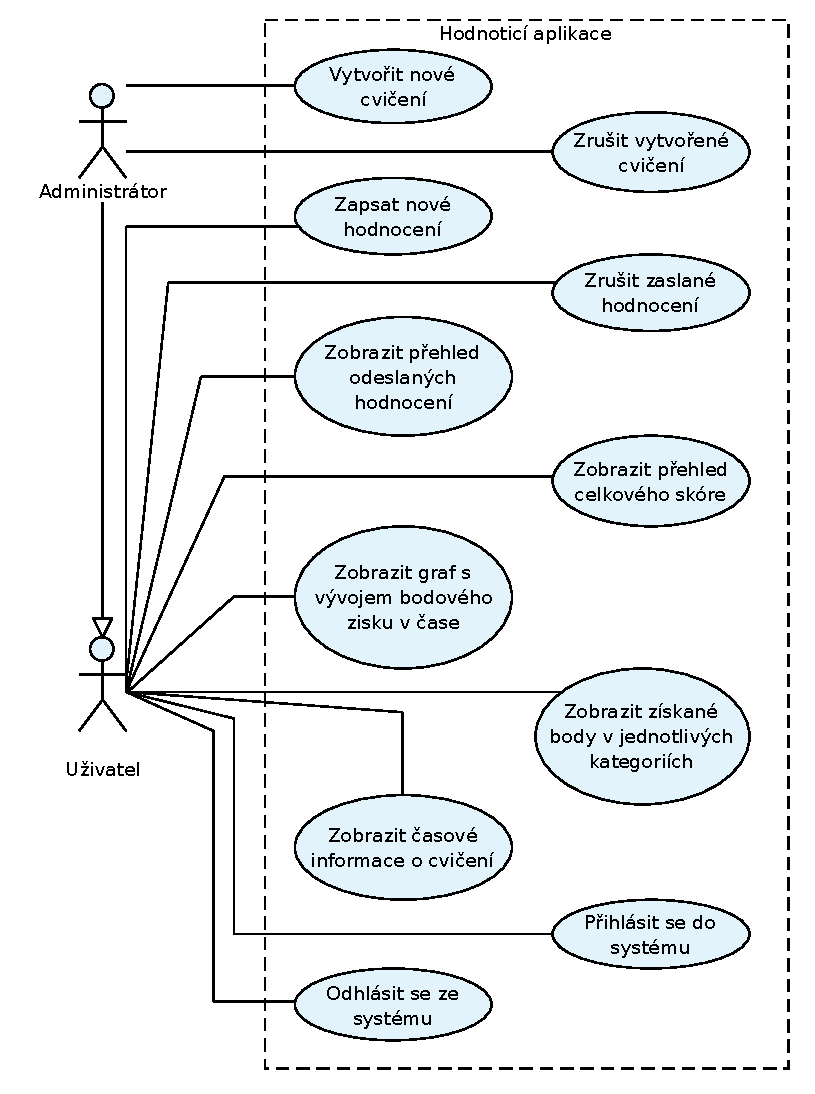
\includegraphics[width=10cm]{images/Use-case-1.eps}
    \caption{Diagram případů užití shrnující veškerou funkcionalitu původní skórovací aplikace.}
    \label{fig:useCase1}
\end{figure}

\section{Model hodnocení účastníků cvičení}
Model pro hodnocení týmů účastnících se cvičení Cyber Czech byl navržen tak, aby týmy získávaly bodovou penalizaci za nedostupnost předem definovaných služeb (dostupnost byla kontrolována automaticky, proto se používá termín automatické hodnocení) a dále týmy získávaly, nebo ztrácely body pomocí manuálně zadaného hodnocení od červeného týmu, bílého týmu, fiktivních uživatelů spravovaného systému a nebo od organizátorů cvičení (zelený tým).

\subsection{Automatické skórování}
Během cvičení byli členové modrého týmu bodově penalizováni za nedostupnost legitimních služeb. Pro kontrolu dostupnosti těchto služeb se využíval monitorovací systém přítomný ve virtuálním prostředí KYPO. V případě nedostupnosti služby byl vložen záznam do fronty v RabbitMQ serveru a aplikace si poté tento záznam načetla a vyhodnotila, zda má dojít k bodové penalizaci a týmu byly případně odečteny body za nedostupnost služby.
\subsection{Manuální skórování}
Kromě bodové penalizace za nedostupnost definovaných služeb bylo v aplikaci možné zadávat i manuální bodové ohodnocení. Toto hodnocení zadávali členové červeného týmu, bílého týmu, členové skupiny legitimních uživatelů systému nebo členové zeleného týmu. Zadávat hodnocení bylo možné jen pro předem definované události, které měly stanovenou dolní a horní bodovou mez. V případě červeného týmu odpovídaly tyto události předem naplánovaným útokům. Naopak v případě bílého týmu nebo legitimních uživatelů se jednalo o události obecné povahy, např. komunikace s modrým týmem.

Manuální hodnocení bylo možné zadávat pomocí formuláře, kde uživatel vybral modrý tým, kterému hodnocení zadává. Dále vybral požadovanou událost, zadal bodové ohodnocení z definovaného intervalu a také mohl hodnocení doplnit slovním komentářem.

\section{Datový model}
\subsection{Popis datového modelu}

Entitně relační diagram na obr. \ref{fig:erdDjango} ukazuje část ze systému pro správu uživatelů, která je součástí Django frameworku a je využívána skórovací aplikací. Nyní blíže popíšu entity, které se v diagramu nachází.

Tabulka $auth\_user$ slouží pro ukládání uživatelských účtů. Sloupec $is\_superuser$ označuje super uživatele, který automaticky získává nejvyšší oprávnění pro správu systému. Atribut $is\_staff$ identifikuje uživatelský účet, který má přístup do administrace, kterou framework Django automaticky vytváří. Zbývající atribut $is\_active$ reprezentuje, zda je možné se k účtu přihlásit.

Tabulka $auth\_group$ slouží pro ukládání uživatelských skupin, které jsou využity pro rozdělení uživatelů do jednotlivých týmů. Tabulka $auth\_user\_groups$ zajišťuje vazbu mezi uživateli a skupinami. Systém pro správu uživatelů dále obsahuje mechanismy pro nastavování oprávnění i na úrovni uživatelských skupin. Skórovací aplikace však těchto vlastností nevyužívá, a proto je pro zjednodušení neuvádím.

\begin{figure}[h!]
    \centering
    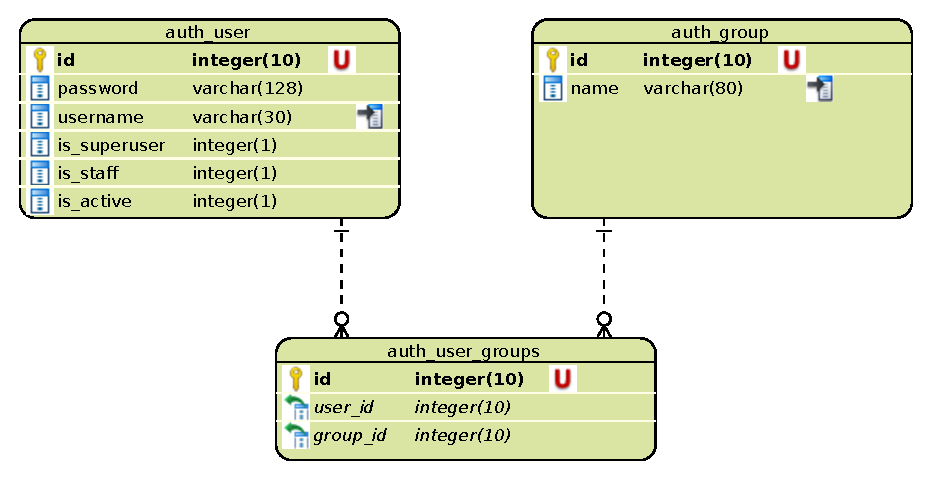
\includegraphics[width=13cm]{images/ERD-django.eps}
    \caption{Entitně relační diagram zachycující strukturu dat v systému správy uživatelů frameworku Django}
    \label{fig:erdDjango}
\end{figure}

Při implementaci předešlé skórovací aplikace byl pozměněn původně navržený datový model a vlivem těchto rozdílů se do databáze zanesly nejrůznější nedostatky. V následujících odstavcích nejdříve popíšu samotný datový model, který je zachycen na obrázku \ref{fig:erdOldApp}. Následně shrnu nedostatky tohoto modelu. 

\begin{figure}[h!]
    \centering
    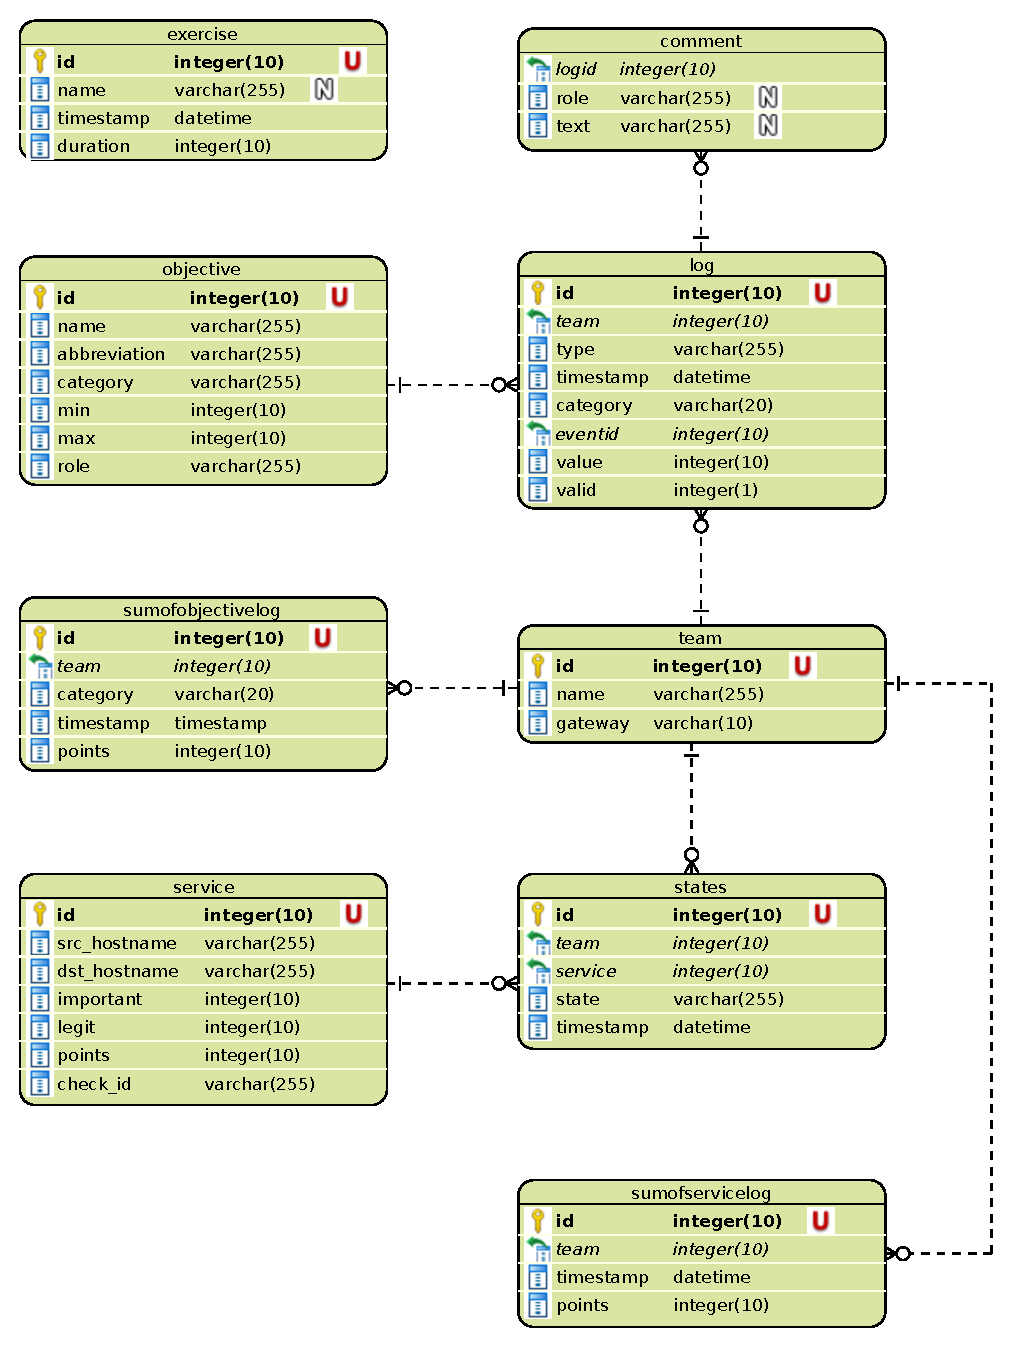
\includegraphics[width=13.5cm]{images/ERD-old-app.eps}
    \caption{Entitně relační diagram popisující datový model původní aplikace}
    \label{fig:erdOldApp}
\end{figure}

Tabulka $Exercise$ obsahovala informaci o vytvořeném cvičení. Do sloupce $timestamp$ se ukládal čas začátku cvičení. Sloupce $duration$ nesl informaci o délce trvání cvičení v celých hodinách a do sloupce $name$ bylo možné z GUI nastavit hodnotu $start$ nebo $stop$, která označovala, zda jde o nastavení času začátku cvičení, nebo ukončení cvičení. S hodnotou $stop$ však aplikace žádným způsobem dále nepracovala, jelikož délka cvičení byla nastavena atributem $duration$. Data, která měla v tomto sloupci uloženou hodnotu $stop$, tedy neměla žádný význam.

Tabulka $Team$ obsahovala informace o týmech účastnících se cvičení. Atribut $gateway$ sloužil pro zadání identifikátoru, který identifikoval hodnoty z automatického skórování pro daný tým.

Tabulka $Objective$ sloužila pro ukládání událostí, za které mělí být účastníci cvičení hodnoceni. Pouze na základě akcí, definovaných v této tabulce, bylo možné zadávat v aplikaci bodové ohodnocení soutěžícím týmům. Každá událost měla uložen svůj název, zkratku, kategorii, minimální a maximální bodové ohodnocení a uživatelskou roli určující, který tým smí hodnocení pro danou událost odeslat. Tento atribut od sebe rozlišoval červený tým, bílý tým, blondýny nebo do něj bylo možné uložit hodnotu, která určovala, že danou událost může hodnotit kdokoliv s přístupem do skórovací aplikace. Atribut $category$ obsahoval číselný identifikátor role, avšak tento sloupec nebyl v aplikaci využit. Při vytvoření záznamu v tabulce $sumofobjectivelog$ se tento sloupec překopíroval do sloupce $category$, ale dále se s touto hodnotou nikde v aplikaci nepracovalo.

Tabulka $log$ obsahovala záznam o samotném zadání hodnocení. U této tabulky došlo k velkému odchýlení od původního návrhu, jelikož měla sloužit pro uložení záznamu jak o automatickém, tak i manuálním skórování. Výhodou původního záměru mělo být usnadnění sledování skóre v čase. Avšak ve výsledné implementaci se do této tabulky ukládala data pouze z manuálního hodnocení. Tabulka obsahovala vazbu na konkrétní tým, typ, který byl vždy nastaven na hodnotu $O$. Dále časovou značku, kategorii, která odpovídala uživatelské roli uložené pro danou událost z tabulky $objective$, referenci na samotnou událost, bodové ohodnocení a na závěr informaci o tom, zda je záznam platný. 

K tabulce $log$ se dále váže tabulka $comment$, do které byl uložen případný slovní komentář k udělenému ohodnocení. Pomocí cizího klíče byla uložena v tabulce reference na daný log.

Účelem tabulky $sumofobjectivelog$ bylo snadné zjištění aktuálního skóre daného týmu. Poslední záznam v této tabulce měl odpovídat skóre, které tým aktuálně má. To znamená, že tabulka musela být aktualizována s každou změnou skóre, tedy například i při smazání chybně zadaného hodnocení. Informace uložená v této tabulce mohla být kdykoliv zjištěna z tabulky $log$ a z tohoto pohledu se tedy jedná o ukládání duplicitní informace.

V tabulce $service$ byl uložen seznam služeb, jejíž dostupnost se během cvičení kontrolovala pomocí automatického skóringu. Tato tabulka obsahovala informaci o zařízení, na kterém je služba provozována, a dále port, na kterém by měla být služba dostupná. Atributy $important$ a $points$ definovaly, jak velkou bodovou ztrátu týmu způsobí nedostupnost této služby. Sloupec $legit$ označoval, zda jde o legitimní službu, která musí být dostupná. Pokud sloupec nebyl nastaven na hodnotu 1, nebyla nedostupnost této služby nijak penalizována. 

Tabulka $states$ obsahovala záznam o zkontrolované dostupnosti nebo nedostupnosti dané služby. Při kontrole dané služby byl v tabulce vytvořen záznam, zda je služba, specifikovaná ve sloupci $service$, dostupná, nebo nedostupná. Stav dostupnosti byl uložen v atributu $state$ pomocí hodnoty $up$ nebo $down$. Dále se ukládal čas provedené kontroly.

Zbývající tabulkou je $sumofservicelog$, která je velice podobná tabulce $sumofobjectivelog$ a v této tabulce je pro každý tým uložen vývoj skóre z automatického hodnocení. Poslední vložený záznam pro daný tým by měl odpovídat aktuální hodnotě skóre z automatického hodnocení.

\subsection{Nedostatky datového modelu}

V původním datovém modelu jsem shledal několik nedostatků. V následujících odstavcích se zaměřím na ty nejvážnější.

V tabulce $sumofservicelog$ neexistuje žádná vazba, ze které by šlo určit, která služba byla nedostupná a způsobila tak bodovou penalizaci. V původním návrhu datového modelu měla být tato informace uložena v tabulce $log$, avšak při implementaci se tato tabulka pro automatické hodnocení nevyužila. 

Nelze snadno sledovat vývoj bodového ohodnocení v čase, jelikož pro přesné zjištění těchto dat je nutné procházet dvě tabulky ($log$ a $sumofservicelog$). Tento nedostatek opět souvisí s nevyužitím tabulky $log$ i pro automatické hodnocení.

Tabulky $sumofservicelog$ a $sumofobjectivelog$ jsou nadbytečné. Potřebné informace by mohly být dostupné v tabulce $log$. Navíc pomocí agregačních dotazů nad touto tabulkou by bylo možné získat celkové skóre v řádu desítek milisekund i nad obrovským množstvím záznamů. Nutnost neustálé aktualizace dat v této tabulce vnáší navíc do aplikace složitější logiku náchylnou na chybu. 

U manuálního hodnocení týmů v tabulce $log$ docházelo k ukládání reference na tabulku $objective$ a dále se ukládala i informace o uživatelské roli, ze které bylo hodnocení zadáno, avšak tuto informaci bylo možné zjistit přímo z vazby na tabulku $objective$.

V datovém modelu se dále vůbec nepočítalo s možností ukládat informace o tom, který uživatel zadal týmu dané hodnocení. Nebylo tedy možné dohledat, kdo je zodpovědný za udělené skóre.

Nedostatkem v relačním návrhu je skutečnost, že pro ukládání dat, která odpovídají údajům uloženým v jiné tabulce, nebylo využito cizích klíčů. Např. v případě uživatelských rolí se ukládala role pouze jako textový název  (tabulka $objective$ a sloupec $role$). Pro využití klauzule $JOIN$ v SQL dotazech je toto nevyhovující.

\section{Nedostatky aplikační a prezentační vrstvy}

Kromě nedostatků v datovém modelu vykazovala aplikace další anomálie, které se projevovaly neočekávanými pády aplikace, případně výpisem chybných dat v aplikaci.

K neočekávanému pádu aplikace docházelo např. při odeslání manuálního hodnocení, kde bodové ohodnocení bylo mimo specifikovaný rozsah. Další chybu způsobovalo odeslání formuláře bez vybraného týmu. Oba případy způsobily pád aplikace, uživateli byla zobrazena chyba a pomocí tlačítka zpět se musel uživatel vrátit na původní stránku.

Chybně se chovala i časomíra, ukazující, kolik času zbývá do konce cvičení. Výpočty s časem nebyly prováděny správně, a tak například po ukončení cvičení docházelo k zobrazení časového údaje se záporným počtem hodin, které zbývají do ukončení cvičení.

Aplikace nedisponovala žádným rozhraním pro správu uživatelských účtů, hodnocených událostí (tabulka $objective$), seznamu služeb (tabulka $services$) nebo například automatického skóre. Uvedená data bylo možné upravovat pouze přímým zásahem do databáze.

\chapter{Návrh nové skórovací aplikace}
V průběhu času začaly vznikat nové funkční požadavky na skórovací aplikaci. Vzhledem k nedostatkům, které původní systém obsahoval, a nedostatečné modularitě celého systému bylo jako nejvýhodnější řešení zvoleno vytvoření zcela nové aplikace. 

Nová aplikace musí plně zachovat původní funkcionalitu a být rozšířena o nové požadavky, ale zároveň musí být opraveny veškeré nedostatky objevené v původní aplikaci. Z tohoto důvodu byla nejdříve provedena revize datového modelu a poté do něj byly zaneseny změny, které vyplynuly z nových požadavků. 

\section{Nové požadavky na skórovací aplikaci}
\subsection{Požadavky na architekturu aplikace}

Jak již bylo nastíněno v úvodu této kapitoly, jeden z hlavních požadavků na novou aplikaci je zajištění větší modularity celého systému. Z tohoto důvodu došlo ke dvěma zcela zásadním změnám.

Bylo rozhodnuto o rozdělení aplikace na samostatnou servisní vrstvu, která pomocí aplikačního programového rozhraní (API) bude poskytovat data prezentační vrstvě. Servisní vrstva skórovací aplikace tedy bude představovat samostatnou aplikaci a k této bude souběžně vyvíjena prezentační vrstva, která bude zpracována opět jako webová stránka za pomocí javascriptového frameworku Angular. Zmíněná webová aplikace bude vyvíjena v rámci jiné bakalářské práce. Pomocí provedeného rozdělení bude zajištěna větší nezávislost samotných systémů a aplikace bude moci lépe využívat moderních principů vývoje webových stránek. Tím je například dynamická aktualizace pouze vybraných částí webové stránky pomocí javascriptu, bez nutnosti načítat opakovaně kompletní webovou stránku. V budoucnu by tento krok mohl dále přinést možnost  snadného napojení i dalších subsystémů na samotnou skórovací aplikaci. Například by mohlo být možné systém propojit s další aplikací, která se stará o přípravu dat pro tvorbu dokumentu se zpětnou vazbou, který dostávají členové modrého týmu po ukončení cvičení, tzv. feedback portlet.

Dalším krokem, který zjednoduší architekturu celé aplikace, je vyčlenění logiky automatického skóringu. Původní aplikace obsahovala skript, který se po spuštění připojil k RabbitMQ serveru a odtud načítal údaje o nedostupnosti služeb, které byly do fronty zapisovány pomocí monitorovacího systému KYPO. Skript následně pomocí předdefinovaných pravidel rozhodoval o bodové penalizaci za nedostupnost služeb a tuto penalizaci ukládal do databáze. Bylo rozhodnuto, že bude celý proces kontroly dostupnosti služeb a vyhodnocování případné bodové penalizace vyčleněn z nové aplikace a bude zajištěn samostatným systémem. Tento systém poté bude pomocí dostupného API zapisovat již pouze informaci o udělené bodové penalizaci do skórovací aplikace.

\subsection{Funkční požadavky}

Během několika ročníků cvičení Cyber Czech se objevila celá řada následujících nových požadavků na aplikaci.

\begin{itemize}
\item Zlepšení správy uživatelských účtů -- původní aplikace neobsahovala žádné nástroje pro správu uživatelů a tato správa musela být prováděna přímo v databázi samotného systému. Nové API by tedy mělo obsahovat funkce pro vytváření a úpravu uživatelů a jejich zařazování do dříve definovaných týmů.
\item Nastavení, pro které týmy může uživatel zadávat hodnocení -- u každého uživatele bude možné nastavit, kterým modrým týmům může zadávat hodnocení. Během cvičení je typické, že určití členové červeného týmu provádí útoky pouze na vybraný modrý tým. Pomocí tohoto nastavení bude tedy možné vytvořit uživatelský účet, který bude moci hodnotit pouze předdefinovaný tým a bude tím sníženo riziko možné chyby při zadávání hodnocení.
\item Vytvoření rozvrhu pro hodnocené události -- jednou ze zásadních novinek nové aplikace bude zobrazení rozvrhu naplánovaných událostí, kde uživatelé skórovací aplikace velice přehledně uvidí, které události by měly být v jakém čase prováděny. Jednotlivým událostem bude možné nastavovat, zda jsou již ve stavu provádění, případně zda událost byla úspěšně, nebo neúspěšně provedena. Bude tedy nezbytné umožnit k událostem ukládat čas, kdy mají být události provedeny. Údaj, který se bude ukládat, bude pouze počet hodin a minut od začátku cvičení, kdy má daná událost nastat. Díky tomu bude možné stanovit různý čas zahájení cvičení a v systému bude uloženo, že daná událost má být provedena například dvě hodiny po zahájení cvičení.
\item Možnost odesílat upozornění na plánované události -- Prezentační vrstva by měla zajistit upozornění uživatele na události, které by měly být právě zahájeny. V servisní vrstvě musí být možné nastavit, zda pro danou událost má takové upozornění být vytvořeno.
\item Používání herního času -- herní čas představuje počet hodin a minut od zahájení cvičení. Pro lepší čitelnost informací v prezentační vrstvě je požadováno, aby servisní vrstva prováděla výpočet herního času na základě nastaveného zahájení cvičení a tento herní čas byl odesílán spolu s daty o hodnocení.
\item Možnost nahrávání souborů k hodnocení – při vytváření hodnocení by mělo být možné nahrávat například snímek obrazovky nebo jiný obrazový, případně textový soubor.
\item Možnost nastavení ikony a dalších rozlišovacích prvků týmu -- aby bylo možné v prezentační vrstvě týmy patřičně rozlišit, byl vznesen požadavek na možnost uložení malé ikony pro každý tým a dále na nastavení barvy, která bude pro daný tým použita při vykreslování grafů.
\end{itemize}

Veškerou novou funkcionalitu systému zachycuje diagram případu užití na obrázku \ref{fig:useCase2}.

\begin{figure}
    \centering
    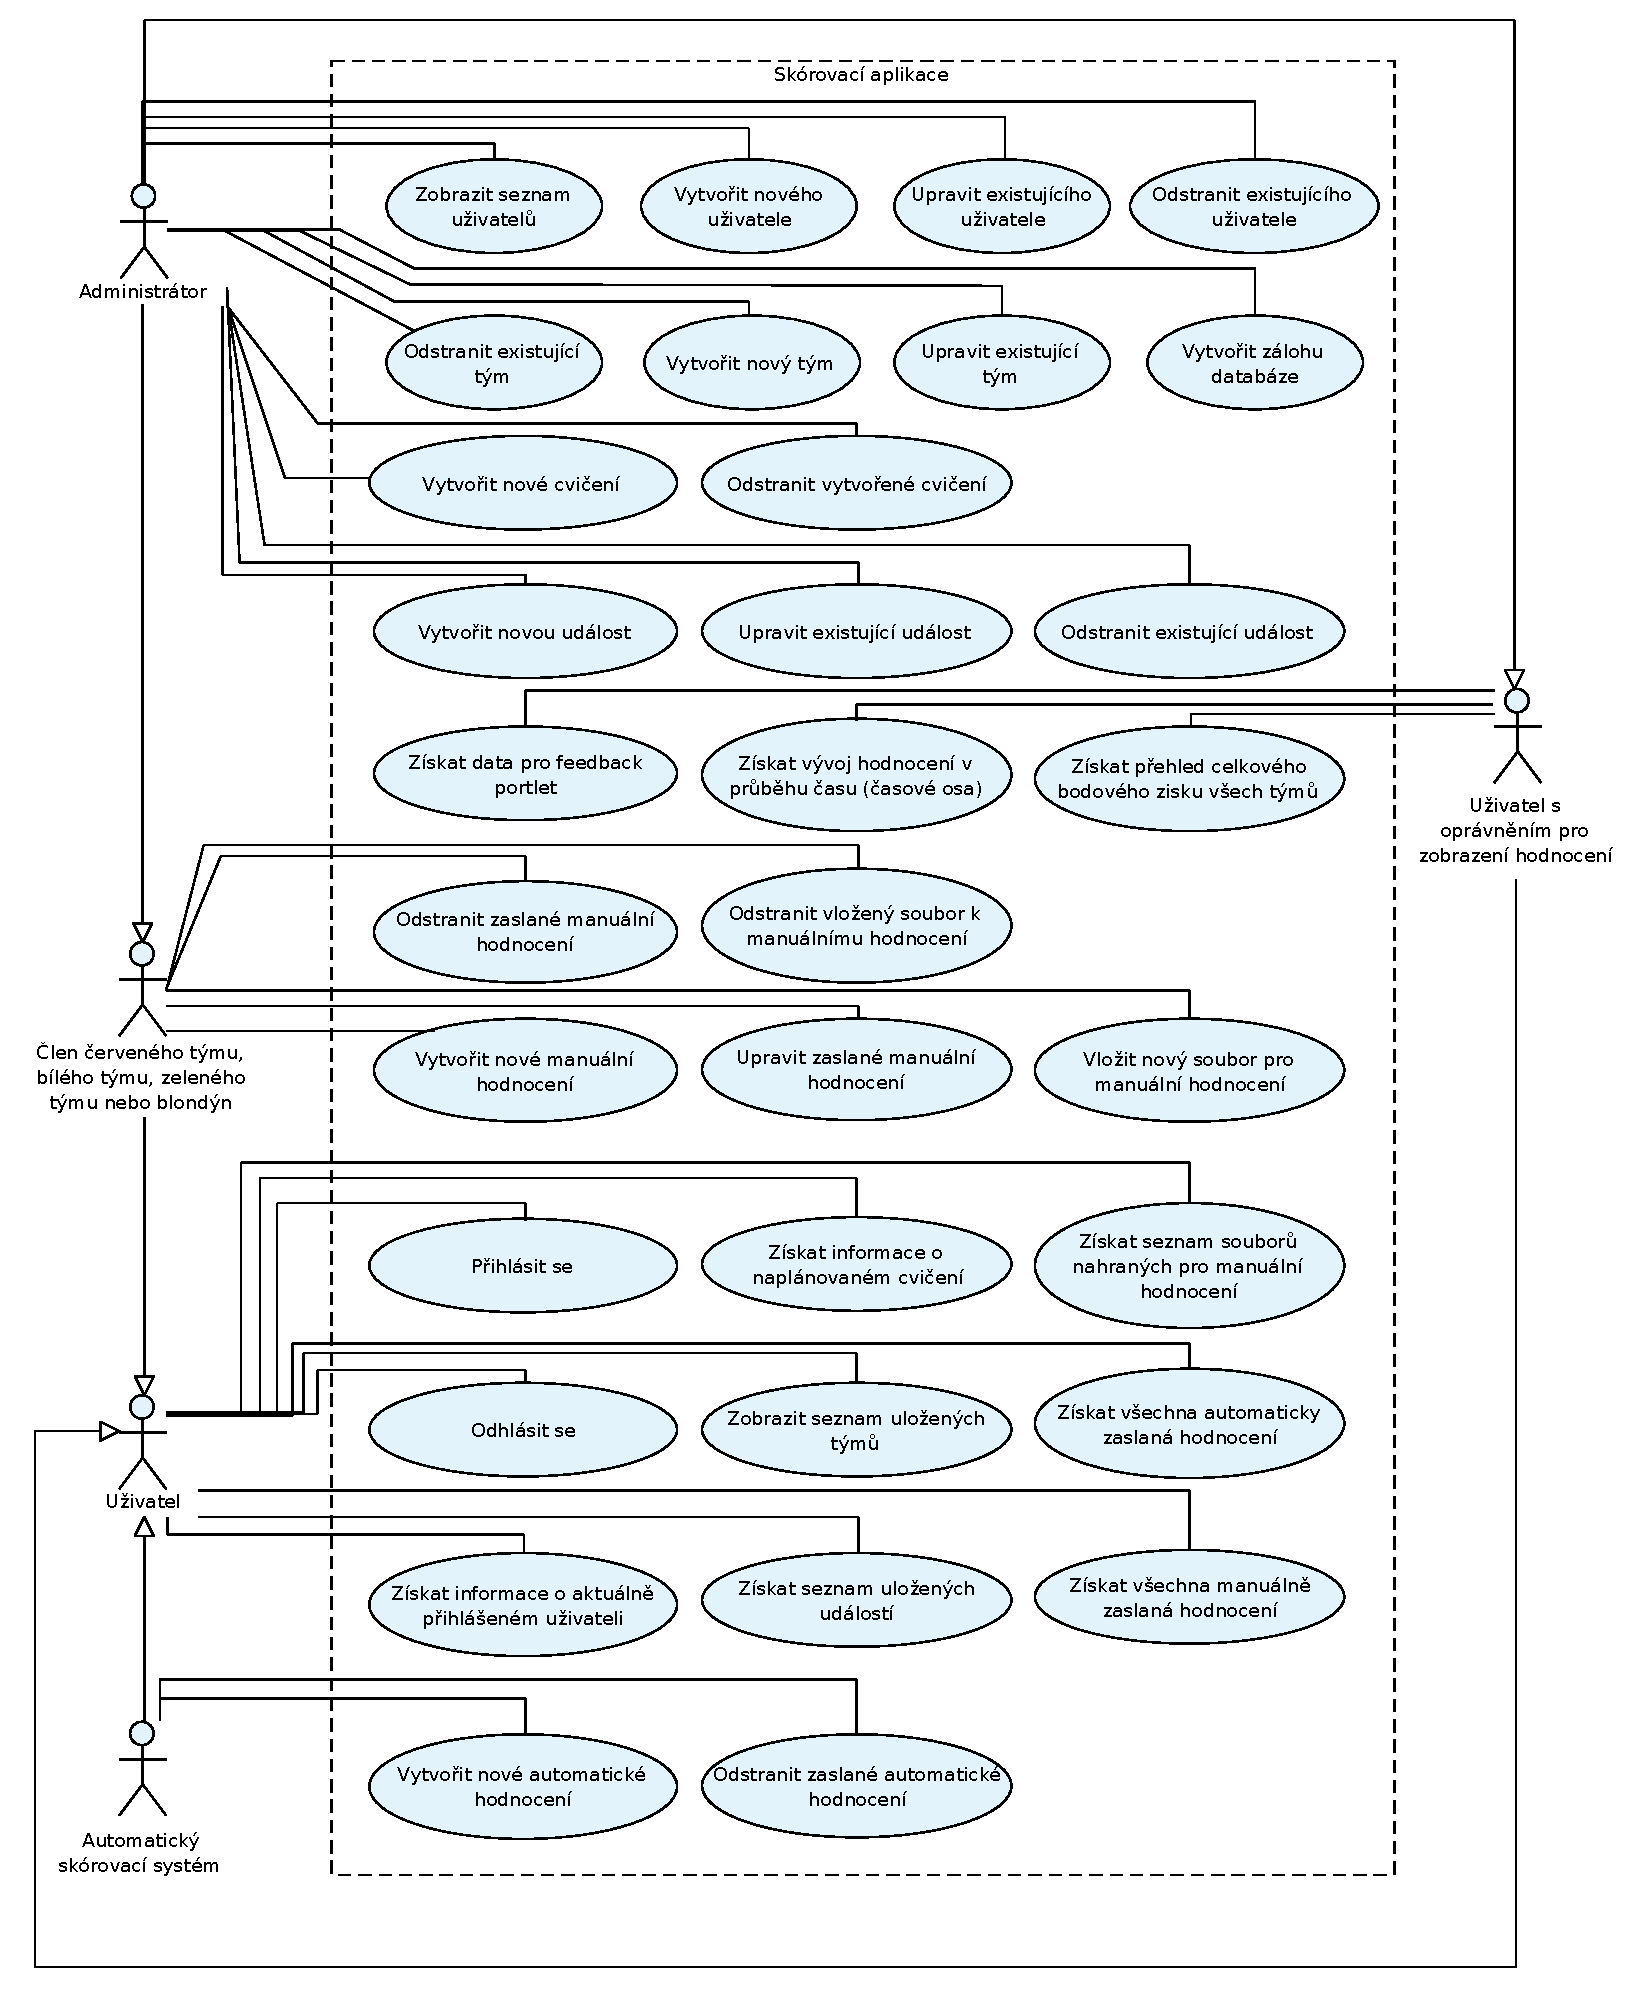
\includegraphics[width=15cm]{images/Use-case-2.eps}
    \caption{Diagram případu užití, který popisuje veškerou funkcionalitu obsaženou v API nové skórovací aplikace}
    \label{fig:useCase2}
\end{figure}

\section{Požadavky na použité technologie}

Původní skórovací aplikace byla implementována pomocí programovacího jazyka Python, pro který existuje velké množství knihovních modulů, mezi než patří i použitý framework Django. Tento systém velice usnadňuje tvorbu webových aplikací a existuje pro něj rozšíření v podobě Django REST framework. Rozšíření je určeno speciálně pro vytváření API a pomocí nástrojů, které obsahuje, je možné efektivně vyvíjet propracované systémy. Výhodou tohoto frameworku je především výborná provázanost s Django ORM systémem, kdy není nutné implementovat například funkce pro ukládání a úpravu dat, jelikož tyto funkce jsou obstarány automaticky. Dále tato nástavba umožňuje snadný převod dat do strojově čitelných formátů (JSON, XML) za použití tzv. serializerů. Nezbytnou součástí frameworku je rozhraní pro vytváření automatických systémových testů pro jednotlivé přístupové body v API.

U jazyka Python dojde k přechodu z verze 2.7 na verzi 3.5, jelikož verze 2.7 je již zastaralá a bylo oznámeno ukončení podpory této verze k roku 2020 \cite{python27}.


\section{Revize datového modelu}

Při revizi původního datového modelu jsem zjistil, že aplikace vykazuje mnohé nedostatky. Zaměřil jsem se především na odstranění duplicity dat a kvalitnější interpretaci ukládaných informací, aby bylo možné sestavovat efektivnější databázové dotazy. Dále jsem se zaměřil na zlepšení v oblasti řízení přístupu uživatelů k datům.

Z pohledu duplicity dat bylo nevyhovující ukládání bodového hodnocení pro daný tým. Duplicita spočívala v tom, že se při každém vložení nového hodnocení informace vložila nejprve do tabulky $logs$ a poté se aktualizovala hodnota se součtem hodnocení pro konkrétní tým v tabulce $sumofobjectivelog$.

V databázovém modelu chyběla identifikace uživatelů zodpovědných za vložený obsah nebo hodnocení. 

V případě ukládání manuálního a automatického hodnocení se jedná o data se stejnou strukturou. Bohužel, v původním návrhu byla tato data ukládána odděleně do dvou tabulek $logs$ a $states$, což vedlo ke složitější logice při sestavování databázových dotazů.

\subsection{Návrh řešení nedostatků datového modelu}
Pro ukládání automatického nebo manuálního hodnocení je navržena jedna společná tabulka, která nese informaci o tom, který tým je hodnocen, kdy k hodnocení došlo a počet udělených bodů. Data, která jsou specifická pro konkrétní typ hodnocení, jsou poté uložena v samostatné tabulce. Mezi těmito tabulkami je vytvořena vazba. Díky tomu je možné snadněji procházet data pouze z jednoho typu hodnocení.

Významnou změnou v datovém modelu bylo vypuštění databázových tabulek, které obsahovaly průběžný součet bodů pro daný tým. Tyto tabulky bylo nutné aktualizovat při každé změně bodového hodnocení. Data o aktuálním bodovém zisku daného týmu bude možné ukládat bez duplicit a zjistit je i bez původních tabulek pomocí agregačních dotazů nad tabulkou, ve které jsou uloženy veškeré záznamy z hodnocení. Tato změna přinese zjednodušení ve výsledné implementaci aplikace.

Pro identifikaci, který uživatel je zodpovědný za zaslané hodnocení, případně další obsah, byl do tabulek $logs$, $files$ a $comments$ přidán atribut pro uložení této informace. Nová aplikace bude využívat autentizačního a autorizačního systému frameworku Django, z tohoto důvodu je do tohoto atributu ukládán cizí klíč na tabulku $auth\_user$, která je součástí frameworku.

\section{Nový datový model}

Datový model samotné aplikace se skládá z 9 databázových tabulek. V následující kapitole se budu zabývat podrobným popisem významu jednotlivých tabulek, definicí atributů a popisu relačních vztahů.

$exercises$ ukládá informaci o naplánovaném cvičení. V tabulce je uložen čas začátku cvičení, délka trvání tohoto cvičení a dále příznak, zda je záznam platný.

$objectives$ je využívána pro ukládání událostí, za které budou členové modrého týmu hodnoceni. Každá událost je tvořena názvem, zkratkou, volitelným popisem a volitelnou fázi, která může být využita v prezentační vrstvě pro seskupování událostí. Dále se v tabulce nachází sloupce pro minimální a maximální bodový rozsah, který je možné použít při zadávání hodnocení dané události a každá událost má uloženou uživatelskou skupinu, která může danou událost hodnotit. Pro možnosti plánování a vytváření rozvrhu událostí slouží sloupec pro uložení času od začátku cvičení, kdy má být událost (typicky útok) provedena a sloupec určující, jak dlouho by událost měla probíhat. V samotné aplikaci je ošetřeno, aby události s nastaveným časem provedení nešly ohodnotit více než jedenkrát pro každý tým. Tímto je zajištěno, aby v rozvrhu událostí bylo možné zobrazit, zda již byla daná událost provedena. 

$teams$ slouží pro ukládání informací o modrých týmech. Každý tým musí mít unikátní název a unikátní identifikátor v prostředí KYPO, pomocí kterého bude možné párovat příchozí hodnocení z automatického skórování. Pro každý tým lze nastavit příznak pro skrytí týmu v tabulce s hodnocením, nebo lze volitelně nastavit vlajku a barvu týmu, která bude využita v prezentační vrstvě.

$teamsJudge$s reprezentuje vazbu M:N mezi tabulkami $teams$ a $auth\_users$ a umožňuje tak kontrolu, zda daný uživatel smí zadávat hodnocení pro daný tým. 

$logs$ představuje společné uložiště pro všechny příchozí druhy hodnocení. Každé hodnocení má společná data, a to tým, kterému je hodnocení uděleno, dále čas udělení hodnocení, počet udělených bodů a autora zaslaného hodnocení. Každý záznam v této tabulce má nastaven příznak, který určuje, zda jde o validní hodnocení, nebo hodnocení, které bylo smazáno. Ve sloupci $type$ je uložena informace o tom, o jaký druh hodnocení se jedná. Rozlišení je provedeno pomocí numerických konstant zadefinovaných ve zdrojovém kódu aplikace.

$automaticLogs$ obsahuje záznamy o zadaném automatickém hodnocení. Každý záznam má uloženou vazbu na záznam ve společné tabulce $logs$. Záznam v tabulce $automaticLogs$ nemůže existovat bez patřičného záznamu v tabulce $logs$. Každé automatické hodnocení má uloženy informace o zařízení, které bylo kontrolováno, o službě, která byla kontrolována a informaci o stavu, v jakém služba byla.

$manualLogs$ obsahuje naopak záznamy z manuálně zadávaného hodnocení. Záznamy v této tabulce opět nemohou existovat bez záznamu v tabulce $logs$. Každé hodnocení má uloženou vazbu na danou událost v tabulce $objectives$ a stav hodnocení, který určuje, zda byla událost provedena úspěšně, neúspěšně, případně  teprve čeká na provedení, nebo je právě prováděna. Tento stav se ukládá rovněž pomocí číselných konstant definovaných v aplikaci.

$files$ slouží pro ukládání souborů k zadanému hodnocení. Každý záznam má tedy referenci na patřičný záznam v tabulce $logs$, cestu k souboru, název souboru a samotného autora souboru.

$comments$ je tabulka pro ukládání komentářů. Stejně jako soubory jsou vázány na konkrétní záznam v tabulce $logs$ a je zde uložena reference na autora komentáře. Uvedené řešení umožňuje do budoucna rozšíření aplikace o možnost diskuze více uživatelů nebo nahrávání souborů v rámci jednoho hodnocení.

Zbývající tabulky $auth\_user$, $auth\_group$ a $auth\_user\_groups$ jsou součástí Django frameworku a v modelu na obrázku \ref{fig:erdNewApp} níže jsou zaneseny pro znázornění, jak bylo tohoto autentizačního a autorizačního systému, poskytovaného frameworkem, využito v datovém modelu.

\begin{figure}
    \centering
    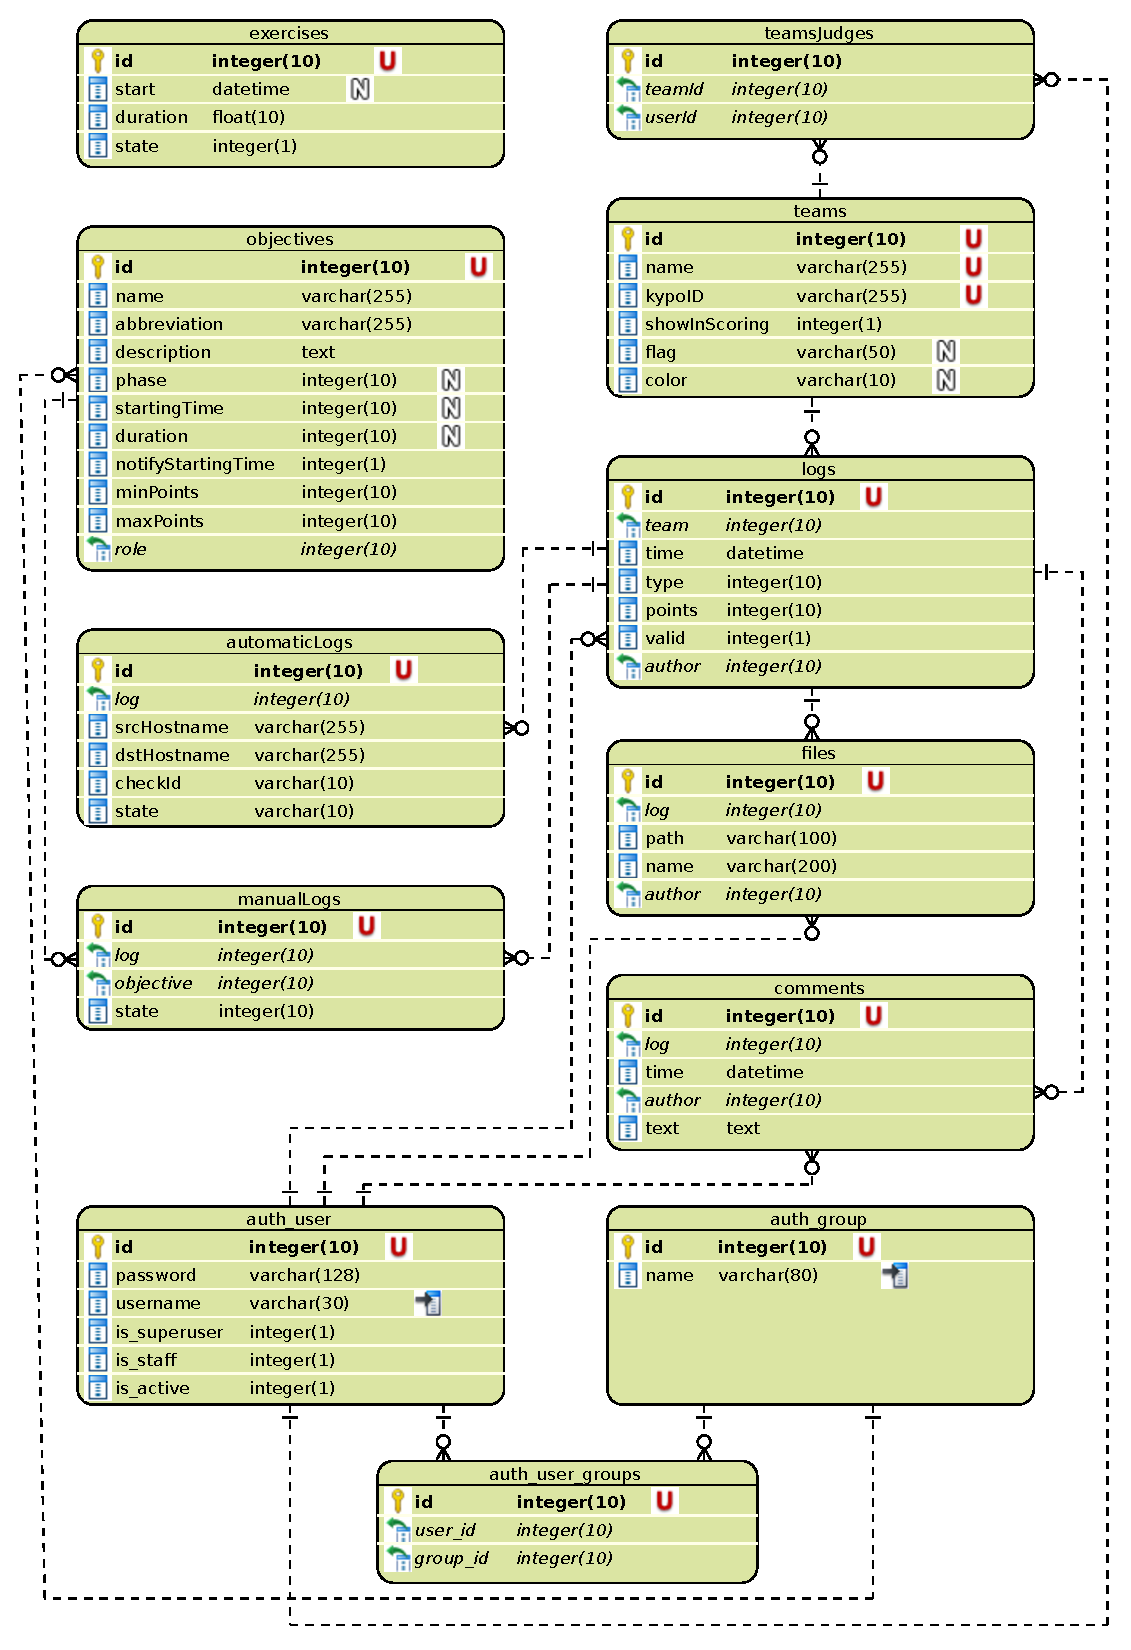
\includegraphics[width=12.5cm]{images/ERD-new-app.eps}
    \caption{Entitně relační diagram mapující kompletní strukturu nového datového modelu}
    \label{fig:erdNewApp}
\end{figure}

\newpage

\section{Návrh API}

Po dokončení revize datového modelu byl vytvořen návrh API pro novou aplikaci. Tento návrh se řídil principy REST (Representational state transfer), což je softwarová architektura, definující sadu pravidel, jakým způsobem bude přistupováno k určitému webovému zdroji a jakým způsobem budou probíhat operace s tímto zdrojem \cite{RoyThomasFielding2000ArchitecturalArchitectures}.
REST architektura byla navržena pro distribuované systémy, ve kterých jsou komponenty systému rozděleny do samostatných celků a tyto mezi sebou komunikují pomocí zasílání zpráv přes počítačovou síť. V našem případě je toto prostředí představováno oddělenou servisní a prezentační vrstvou a pro komunikaci je využit HTTP protokol.  Dle principů REST by webový zdroj měl podporovat operaci čtení, vytváření, upravování a mazání, tedy tzv. CRUD\footnote{Zkratka shrnující čtyři základní operace s daty. Vytvoření (create), čtení (read), úprava (update) a mazání (delete).}. V případě HTTP protokolu se využívá metody GET pro získání dat, POST pro vytváření dat, PUT pro úpravu již existujících dat a DELETE pro mazání dat. Dále tato architektura popisuje, jakým způsobem by měla být data reprezentována ve strojově čitelném formátu. \cite{RoyThomasFielding2000ArchitecturalArchitectures}

Při návrhu API jsem využil online nástroje Swagger\footnote{www.swagger.io}, který generuje velice přehlednou dokumentaci pro API a umožňuje její sdílení i dalším vývojářům.

Následující text obsahuje pouze stručný přehled, který má za úkol nastínit strukturu vytvořeného API. Kompletní dokumentace s přesným popisem odesílaných a přijímaných dat se nachází v elektronických přílohách práce.

\renewcommand\labelitemii{$\square$}
\begin{itemize}
    \item $/users$
    \begin{itemize}
        \item $GET$ -- získání seznamu všech uživatelů
        \item $POST$ --  vytvoření nového uživatele
    \end{itemize}
    
    \item $/users/{user}$
    \begin{itemize}
        \item $GET$ -- získání detailu uživatele
        \item $PUT$ -- upravení existujícího uživatele
        \item $DELETE$ -- odstranění existujícího uživatele
    \end{itemize}
    
    \item $/teams$
    \begin{itemize}
        \item $GET$ -- získání seznamu všech týmů
        \item $POST$ --  vytvoření nového týmu
    \end{itemize}
    
    \item $/teams/{team}$
    \begin{itemize}
        \item $GET$ -- získání detailu týmu
        \item $PUT$ -- upravení existujícího týmu
        \item $DELETE$ -- odstranění existujícího týmu
    \end{itemize}
    
    \item $/exercises$
    \begin{itemize}
        \item $GET$ -- získání informací o naplánovaném cvičení
        \item $POST$ -- vytvoření nového cvičení
    \end{itemize}
    
    \item $/objectives$
    \begin{itemize}
        \item $GET$ -- získání seznam všech událostí
        \item $POST$ --  vytvoření nové události
    \end{itemize}
        
    \item $/objectives/{objective}$
    \begin{itemize}
        \item $GET$ -- získání detailu události
        \item $PUT$ -- upravení existující události
        \item $DELETE$ -- odstranění existující události
    \end{itemize}
        
    \item $/charts/timeline$
    \begin{itemize}
        \item $GET$ -- získání časové osy s jednotlivými změnami bodového hodnocení
    \end{itemize}
        
    \item $/charts/score$
    \begin{itemize}
        \item $GET$ -- získání celkového skóre
    \end{itemize}
        
    \item $/logs/automatic$
    \begin{itemize}
        \item $GET$ -- získání seznamu všech automatických hodnocení
        \item $POST$ --  vytvoření nového automatického hodnocení
    \end{itemize}
        
    \item $/logs/automatic/{log}$
    \begin{itemize}
        \item $GET$ -- získání detailu automatického hodnocení
        \item $DELETE$ -- odstranění existující události
    \end{itemize}
            
    \item $/logs/manual$
    \begin{itemize}
        \item $GET$ -- získání seznamu všech manuálních hodnocení
        \item $POST$ --  vytvoření nového manuálního hodnocení
    \end{itemize}
            
    \item $/logs/manual/{log}$
    \begin{itemize}
        \item $GET$ -- získání detailu manuálního hodnocení
        \item $PUT$ -- upravení existujícího hodnocení
        \item $DELETE$ -- odstranění existujícího hodnocení
    \end{itemize}
            
    \item $/logs/manual/{log}/files$
    \begin{itemize}
        \item $GET$ -- získání seznamu všech souborů pro dané manuálních hodnocení
        \item $POST$ -- vytvoření nového souboru pro dané hodnocení
    \end{itemize}
            
    \item $/logs/manual/{log}/files/{file}$
    \begin{itemize}
        \item $DELETE$ -- odstranění existujícího souboru
    \end{itemize}
            
    \item $/export/database$
    \begin{itemize}
        \item $GET$ -- získání odkazu pro stažení zálohy databáze
    \end{itemize}
                
    \item $/export/feedback$
    \begin{itemize}
        \item $GET$ -- získání dat pro feedback portlet (slouží pro přípravu dokumentů se zpětnou vazbou pro členy modrého týmu)
    \end{itemize}

\end{itemize}


\chapter{Implementace nové skórovací aplikace}

\section{Struktura projektu}
Pro implementaci byl využit Framework Django ve spojení s Django REST framework. Díky zvoleným nástrojům lze vytvářet přehledný a strukturovaný kód. V následujících kapitolách popíšu nejdůležitější části struktury nově vytvořené aplikace.

\subsection{Adresářová struktura}
V hlavním adresáři aplikace se nachází soubor $manage.py$. Soubor slouží pro spouštění příkazů frameworku Django, tedy například spuštění vývojového webového serveru nebo automatických testů. Adresářová struktura je rozdělena na dva samostatné adresáře $scoring$ a $cyberex\_api$.

Adresář $scoring$ obsahuje konfigurační soubor $settings.py$, ve kterém se nachází veškeré nastavení aplikace. V souboru $globals.py$ je zadefinována hodnota výchozího bodového skóre každého týmu. $urls.py$ obsahuje routovací pravidla, pomocí kterých se příchozí požadavky předávají jednotlivým modulům.

Zmíněné příchozí požadavky jsou dle modulů rozděleny podle následujícího přehledu.

\begin{itemize}
    \item $api/v1/$ -- modul skórovací aplikace
    \item $api\-auth/v1/$ -- modul zajišťující autentizaci
    \item $admin/$ -- modul administrace, která je generována frameworkem
\end{itemize}

Adresář $cyberex\_api$ obsahuje veškeré zdrojové kódy skórovací aplikace. Adresářová struktura je následující.

\begin{itemize}
    \item $admin.py$ -- konfigurace pro automaticky generovanou administraci
    \item $helpers.py$ -- pomocné funkce, např. pro počítání herního času k záznamům o hodnocení
    \item $models.py$ -- definice databázového modelu pro ORM systém, viz kapitola \ref{model}
    \item $permissions.py$ -- pravidla autorizačního systému
    \item $serializers.py$ -- soubor tříd zajišťující převod dat do strojově čitelného formátu, viz kapitola \ref{serializer}
    \item $tests.py$ -- automatické testy
    \item $urls.py$ -- definice routovacích pravidel, na základě příchozího požadavku je každý požadavek předán správné funkci v souboru $views.py$
    \item $views.py$ -- soubor tříd, které obsluhují příchozí požadavky, viz kapitola \ref{radic}
\end{itemize}

\subsection{Model}
\label{model}
Framework Django obsahuje propracovaný ORM systém. Veškeré datové modely jsou popsány v souboru $models.py$ a na základě těchto definic je automaticky vygenerována struktura databáze. Model je pouze univerzálním popisem datové struktury, která je nezávislá na použitém databázovém systému. Podporované databázové systémy jsou PostgreSQL, MySQL, SQLite a Oracle. Framework sám spravuje schéma databáze a sestavuje dotazy podle zvoleného databázového systému.

Každá entita je reprezentována samostatnou třídou a může být rozšířena o vlastní metody. Uvedený přístup byl vhodný například při implementaci funkce, která získá pro entitu týmu všechna vložená hodnocení. Tímto je zachována lepší strukturu kódu, jelikož metody, které se starají pouze o získání dat, jsou stále zapsány v modelu.

\subsection{Serializace dat}
\label{serializer}
V systému jsou databázová data reprezentována pomocí entit ORM systému, pro jejich převod do strojově čitelného formátu slouží speciální třídy v souboru $serializers.py$. Pomocí těchto tříd lze však provést i opačný proces, tedy ze strojově čitelného formátu vytvořit nebo upravit entitu. Pomocí mapování na ORM datový model entity je možné realizovat, aby tento proces probíhal zcela automaticky. Programátor však může i nadále do tohoto procesu zasáhnout implementací vlastní metody pro ukládání či editaci. Implementace vlastních metod jsem využil pro ukládání záznamu o hodnocení, kdy se ukládají data do dvou různých databázových tabulek a není tak možné využít generického chování funkcí pro ukládání.

\subsection{Řadič}
\label{radic}
Všechny příchozí požadavky na URL adresu $/api/v1$ jsou pomocí routovacích pravidel předány patřičným funkcím v souboru $views.py$. Tyto metody představují řídící logiku celé aplikace. V případě požadavků na získání informací funkce provede načtení dat z modelu. Následuje předání dat do serializační metody a vzniklý výstup je odeslán v odpovědi serveru. Funkce zajišťuje při požadavcích na vytváření, úpravu nebo mazání záznamů předání přijatých dat do serializační metody. V případě validační chyby dat se funkce postará o vygenerování chybového hlášení. Pokud je nový záznam úspěšně vytvořen nebo upraven, odešle funkce v odpovědi serveru tento záznam.

\section{Instalace a spouštění aplikace}
Aplikace pro svůj běh vyžaduje interpretr jazyka Python ve verzi 3.5 a instalaci několika dalších modulů. Abych zajistil co nejjednodušší instalaci těchto závislostí, rozhodl jsem se využít nástroje Pipenv\footnote{www.pipenv.readthedocs.io}. V následujících kapitolách popíšu použití tohoto nástroje a způsob, jakým byla aplikace distribuována mezi další vývojáře.

\subsection{Řešení závislostí pomocí nástroje Pipenv}
Nástroj Pipenv v sobě spojuje dvě důležité funkcionality. První je správce balíčků, pomocí kterého je možné snadno definovat všechny potřebné závislosti aplikace a následně je jednorázově nainstalovat jediným příkazem. Druhou funkcionalitou je nástroj pro spouštění softwaru v uzavřeném prostředí, které je nakonfigurováno podle definovaných závislostí. Díky tomu je možné v jednom operačním systému spouštět programy pro rozdílné verze jazyka Python a odlišné verze modulů tohoto jazyka.

Veškeré závislosti jsou definovány v souboru $Pipfile$, kde se nachází požadovaná verze jazyka Python a seznam vyžadovaných modulů. Pro spuštění je nutné mít na počítači nainstalován interpretr jazyka Python a nástroj Pipenv. Pomocí příkazu programu Pipenv lze nainstalovat veškeré závislosti.

\begin{lstlisting}
pipenv install
\end{lstlisting}

Pomocí dalšího příkazu lze již spustit samotnou aplikaci.

\begin{lstlisting}
pipenv run runserver
\end{lstlisting}

Příkaz \lstinline[columns=fixed]{pipenv run runserver} je alias definovaný v souboru $Pipfile$ a reprezentuje příkaz \lstinline[columns=fixed]{python manage.py runserver}. Příkaz zapne vývojový server frameworku Django.

Díky použitým nástrojům je spuštění aplikace velice snadné, ale je zde několik dalších nedostatků. Instalace se skládá z několika kroků, při kterých může dojít k chybě. V nainstalované aplikaci neexistují žádná testovací data, včetně uživatelských účtů a vývojový server spouštěný při lokální instalaci se liší od serveru, který je používán v produkčním prostředí v KYPO. Z těchto důvodů jsem se rozhodl pro využití nástroje Vagrant\footnote{www.vagrantup.com}, který za pomocí virtualizace spustí a nakonfiguruje nový virtuální počítač se skórovací aplikací.

\subsection{Spuštění aplikace ve virtuálním prostředí}

Pro zprovoznění aplikace je nezbytné mít k dispozici počítač podporující virtualizaci a dále nainstalované programy VirtualBox\footnote{www.virtualbox.org} a Vagrant. Pomocí jediného příkazu poté dojde ke spuštění virtuálního počítače, na který bude předinstalován operační systém Linux a do tohoto systému budou následně nainstalovány veškeré programy a balíčky nutné pro fungování aplikace. Po připravení prostředí pro běh systému jsou spuštěny další příkazy, které provedou vytvoření uživatelských účtů, ale také vytvoření testovacích dat, aby bylo možné spuštěnou aplikaci ihned využívat. 

Prostředí ve virtuálním počítači je nakonfigurováno tak, aby se co nejvíce blížilo produkčnímu prostředí v KYPO. Jako webový server se používá Apache2, který je nakonfigurován tak, aby komunikoval pomocí šifrovaného protokolu HTTPS. Aplikace s webovým serverem komunikuje pomocí WSGI (Web Server Gateway Interface). WSGI představuje jednotné rozhraní pro komunikaci webových serverů a aplikací naprogramovaných v jazyce Python.

Jako relační databázový systém se využívá SQLite, který byl zvolen převážně kvůli svojí jednoduchosti.

\section{Optimalizace SQL dotazů}

Aplikace získává při volání koncového bodu $/charts/score$ v API aktuální výsledky bodů z automatického skórování nad tabulkou $logs$. Během jednoho cvičení může být vygenerováno až 10000 záznamů hodnocení, a tak aplikace musí být schopna pracovat s velkými počty záznamů. Testováním aplikace se ukázalo, že ORM systém je pro operace nad tímto množstvím dat nevhodný a získávání skóre trvalo řádově několik sekund. V tomto případě se ukázalo jako efektivní využít agregačních SQL dotazů. 

Konkrétně pro získání celkového bodového zisku z automatického skóringu byl použit následující SQL dotaz.

\begin{markdown*}{%
  fencedCode,
}
```
SELECT team_id, SUM(points) FROM logs 
WHERE type = 2 AND valid = 1 
GROUP BY team_id
```
\end{markdown*}

Dotaz využívá funkce $SUM$ pro získání součtu bodů a klauzule $GROUP\ BY$, pro seskupení dat podle identifikátorů jednotlivých týmů. Výběr dat je omezen pouze na validní záznamy z automatického skórování.

Všechny změny bodového skóre v čase se získávají pomocí volání API $/charts/timeline$. Vzhledem k tomu, že tyto hodnoty se opět berou z výše uvedené tabulky $logs$, naráží tato operace opět na limity ORM systému. S přihlédnutím ke skutečnosti, že automatický skórovací systém vkládá do aplikace záznamy o nedostupnosti služeb v dávkách (např. 4 záznamy ve stejný okamžik), jsem se rozhodl využít opět agregační dotaz, který takové záznamy spojí do jednoho a zrychlí tak získávání záznamů a sníží se datový objem dat.

Výsledný SQL dotaz má nasledující podobu.

\begin{markdown*}{%
  fencedCode,
}
```
SELECT team_id, time, SUM(points) FROM logs 
WHERE valid = 1 
GROUP BY strftime('%s', time), team_id 
ORDER BY time
```
\end{markdown*}

V dotazu dochází pomocí klauzule $GROUP\ BY$ k seskupení dat, která mají stejný čas vložení. Opět je využito funkce $SUM$ pro získání celkové sumy bodů.

\section{Automatické testování}

Nedílnou součástí celého projektu jsou automatické systémové testy, které testují softwarovou aplikaci jako celek, zda se chová dle požadavků \cite{difSysTest}.

Díky svojí komplexitě mohou testy odhalit chybné chování na kterékoliv vrstvě aplikace. Příkladem systémového testu je vložení nového záznamu do systému pomocí API a následné provedení kontroly, zda odpověď serveru obsahuje očekávaná data včetně kontroly správného uložení dat v databázovém systému.

Pro implementaci testů byly využity knihovny obsažené v Django REST framework. Pomocí dostupných funkcí je možné sestavit HTTP požadavek, který bude odeslán na spuštěný vývojový server. Po odeslání požadavku je možné provést kontrolu, zda data obdržená v odpovědi serveru odpovídají očekávaným datům. V případě vytváření, úpravy, nebo mazání dat se zároveň provádí i kontrola dat v databázovém systému. 

Celkem bylo implementováno 57 testů. Pro každý existující koncový bod API a každou dostupnou HTTP metodu existuje minimálně jeden test. Pro metody POST a PUT existují typicky varianty testu s validními a nevalidními daty. Testy se nachází v souboru $tests.py$ v adresáři $cyberex\_api$ a jejich spuštění je možné provést v příkazové řádce, spuštěním příkazu $test$ frameworku Django.

Výše uvedené testy jsem využíval pro ověření funkčnosti celého systému po provedení úprav. V praxi je vhodné ověřovat testováním funkčnost softwaru před každou změnou na produkčním prostředí.

\section{Reálné nasazení aplikace na Cyber Czech 2018}



\chapter{Závěr}

\printbibliography[heading=bibintoc] %% Print the bibliography.

\end{document}
